\chapter{Исследовательская часть}

В данном разделе будут приведён пример работы программы, а также проведён сравнительный анализ многопоточной реализации и однопоточной

\section{Технические характеристики}

Технические характеристики устройства, на котором выполнялись замеры времени работы реализации алгоритма статической раздачи информации, представлены далее:

\begin{itemize}
	\item операционная система Mac OS Monterey Версия 12.5.1 (21G83) \cite{macos} x86\_64;
	\item память 16 ГБ;
	\item четырёхъядерный процессор Intel Core i7 с тактовой частотой 2,7 ГГц \cite{intel}.
\end{itemize}

При тестировании ноутбук был включен в сеть электропитания. Во время замеров и нагрузочного тестирования ноутбук был нагружен только встроенными приложениями окружения, а также системой тестирования.

\section{Демонстрация работы программы}

На рисунке \ref{img:example} представлен результат работы программы: разработанное программное обеспечение позволяет раздавать статический файл большого объёма -- страницу в Википедии о Российской федерации, эта страница открыта в браузере, она загружена через локальное доменное имя с указанным портом.

\img{100mm}{example}{Пример работы программы}
\clearpage

\section{Время выполнения алгоритмов}

Для проведения нагрузочного тестирования и замера времени обработки запросов используется утилита wrk.
Нагрузочное тестирование будет производиться в течение 30 секунд с 12 потоков и с указанным числом соединений, результаты (количество обработанных запросов в секунду -- requests per second, или rps, к количеству открытых соединений).

Результаты тестирования приведены в таблице \ref{tbl:rps}.
\begin{table}[h]
	\begin{center}
		\begin{threeparttable}
		\caption{Результаты нагрузочного тестирования}
		\label{tbl:rps}
		\begin{tabular}{|c|c|c|c|}
			\hline
			Количество соединений, шт.& 1 поток, rps&  8 потоков, rps &  16 потоков, rps \\
			\hline
			12 & 537 & 544 & 550 \\ 
			\hline
			40 & 291 & 434 & 546 \\ 
			\hline
			80 & 189 & 387 & 543 \\ 
			\hline
			120 & 147 & 360 & 533 \\ 
			\hline
			160 & 117 & 319 & 514 \\ 
			\hline
			200 & 86 & 220 & 506 \\ 
			\hline
		\end{tabular}
		\end{threeparttable}
    \end{center}
\end{table}

На рисунке \ref{img:graph_rps} приведены графические результаты нагрузочного тестирования.

\begin{figure}[h]
	\begin{center}
		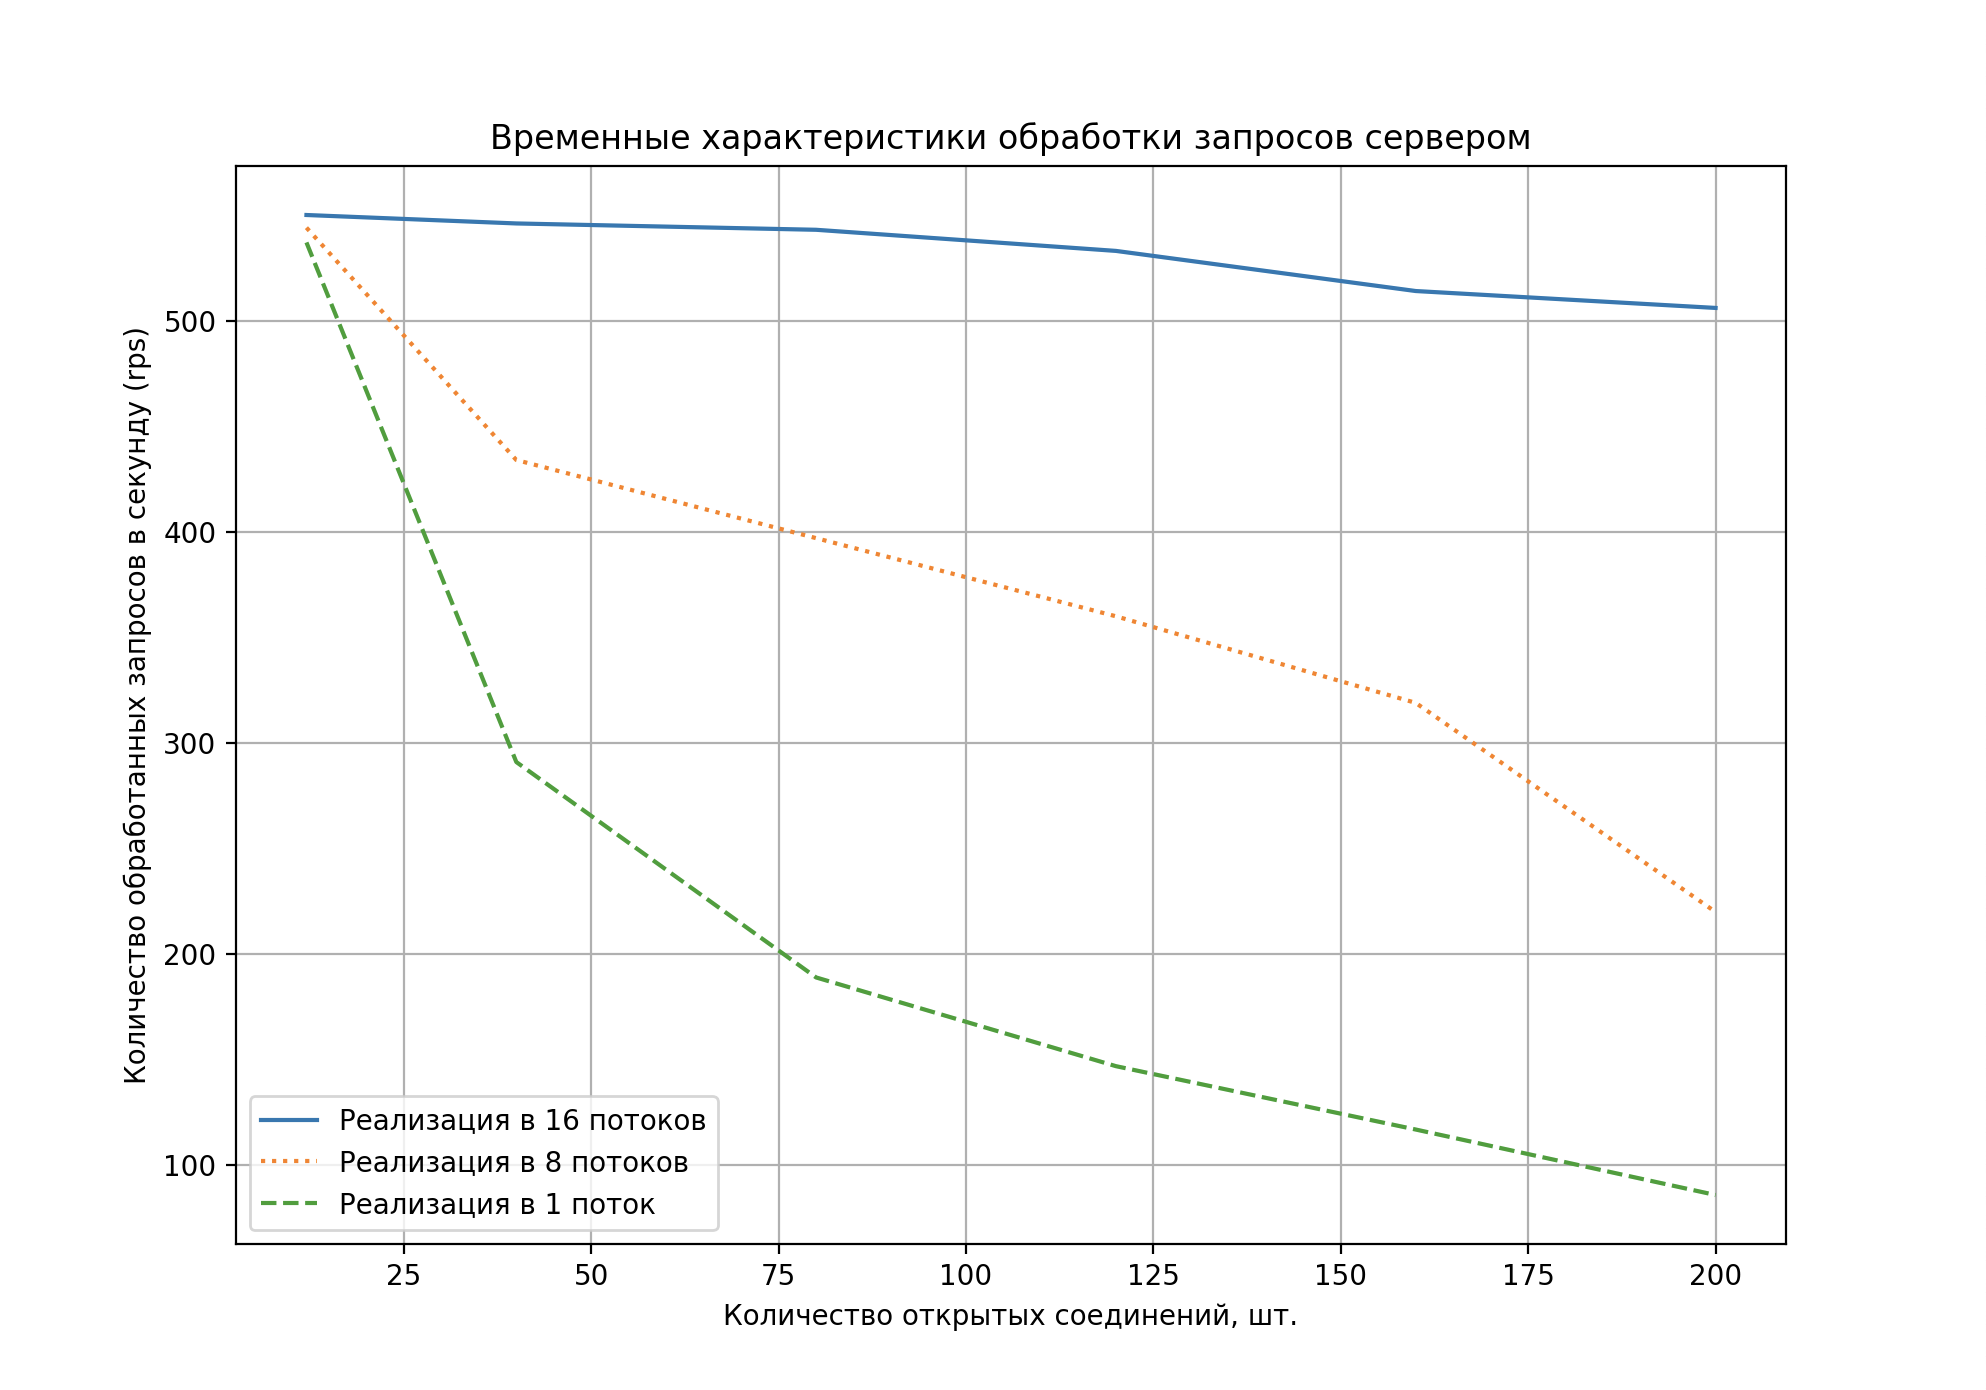
\includegraphics[width=120mm]{graph_rps}
	\end{center}
	\caption{Результаты нагрузочного тестирования}
	\label{img:graph_rps}
\end{figure}
Таким образом, при увеличении числа открытых соединений до 200 в течении 30 секунд реализация с использованием 16 потоков одновременно оказалась более, чем в 6 раз эффективнее реализации с одним потоком, а с использованием 8 потоков -- почти в 3 раза эффективнее.

\section*{Вывод}
Исходя из полученных результатов, при увеличении нагрузки на сервер (например, при увеличении числа открытых соединений) реализация с большим количеством потоков показала наилучший результат. Так, реализация с использованием 16 потоков оказалась более чем в 6 раз эффективнее реализации с одним потоком.
В целом, использование многопоточности показало значительный прирост количества обработанных запросов в секунду, в частности при количестве открытых запросов больше, чем 20.